\documentclass{article}
\usepackage[utf8]{inputenc}
\usepackage[T1]{fontenc}
\usepackage[export]{adjustbox}
\usepackage{mathtools,amsthm,amssymb,icomma,upgreek,xfrac,enumerate, bbm,titlesec,lmodern,polski,derivative,geometry,multicol,titling,graphicx,url,amsmath,caption,lipsum,float,longtable,booktabs}
\usepackage[table,xcdraw]{xcolor}
\usepackage[hidelinks,breaklinks,pdfusetitle,pdfdisplaydoctitle]{hyperref}
\setlength{\droptitle}{-1cm}
\mathtoolsset{showonlyrefs,mathic}
\title{Pakiety statystyczne raport 2}
\author{Adam Wrzesiński, Joanna Kołaczek}
\date{18.07.2022}
\newtheoremstyle{break}
{\topsep}{\topsep}%
{\normalfont}{}%
{\bfseries}{}%
{\newline}{}%
\theoremstyle{break}
\newtheorem{zadanie}{Zadanie} 
\newtheorem*{rozwiazanie}{Rozwiązanie}

\titleformat*{\section}{\LARGE\bfseries}
\titleformat*{\subsection}{\Large\bfseries}
\titleformat*{\subsubsection}{\large\bfseries}
\titleformat*{\paragraph}{\large\bfseries}
\titleformat*{\subparagraph}{\large\bfseries}

%% KOMENDY:
\newcommand*{\e}{\mathrm{e}}
\newcommand{\hyline}[2]{%
	$#1$\> --\kern.5em #2 \\}


%% OPERATORY:
% `\diff` od „differential”, czyli odpowiednika słowa „różniczka” w języku
% angielskim.
\DeclareMathOperator{\diff}{d\!}
\newcommand{\indep}{\perp \!\!\! \perp}
\DeclareMathOperator{\EX}{\mathbb{E}}
\newcommand*{\E}{\mathrm{e}}



\begin{document}
	\maketitle
	\tableofcontents
	\clearpage
	
\section{Wstęp}
	
	Niniejszy raport powstał na potrzeby realizacji laboratorium z Pakietów Statystycznych, prowadzonych przez dr inż. XXXX, do wykładu dr inż. Andrzeja Giniewicza. 
	
	Będziemy testować hipotezy statystyczne dla wartości średniej i wariancji w rodzinie rozkładów normalnych. Zobrazujemy także obszary krytyczne, wyznaczymy p-wartości oraz prawdopodobieństwo wystąpienia błędów I i II rodzaju. Życzymy miłej lektury.
	
	\section{Transformata Sinh-arcsinh}
	Przy generowaniu rozkładu normalnego, musimy ustalić parametr położenia $\mathbf{\mu}$ (dla rozkładu normalnego jest to średnia) oraz parametr skali $\mathbf{\sigma}$ (w tym przypadku będzie to odchylenie standardowe). Transformata sinh-arcsinh rozkładu normalnego wprowadza nowe parametry, które kontrolują asymetrię $\mathbf{\nu}$ i ciężkość ogonów $\mathbf{\tau}$. Dane cztery parametry definiują rozkład normalny Sinh-arcsinh jako:
	$$X = \mu + \sigma \cdot \sinh \left[ \frac{\sinh^{-1}(Z)+\nu}{\tau}\right],$$
	gdzie $Z$ jest zmienną losową z standardowego rozkładu normalnego oraz:
	$$\sinh(x) = \frac{\e^x + \e^{-x}}{2}, \quad \sinh^{-1}(x) = \log(x+\sqrt{1+x^2}).$$
	 Dystrybuanta rozkładu Sinh-arcinh zastosowanego na rozkład normalny wygląda następująco:
	 $$F(x; \mu, \sigma, \nu, \tau) = \phi \left(\sinh \left(\tau \sinh^{-1} \left(\frac{x-\mu}{\sigma}\right)-\nu\right)\right).$$
	 gdzie $\phi$ do dystrybuanta standardowego rozkładu normalnego $\mathcal{N}(0,1)$

	\begin{figure}[H]
		\begin{center}
			\begin{minipage}{0.4\linewidth}
				\centering
				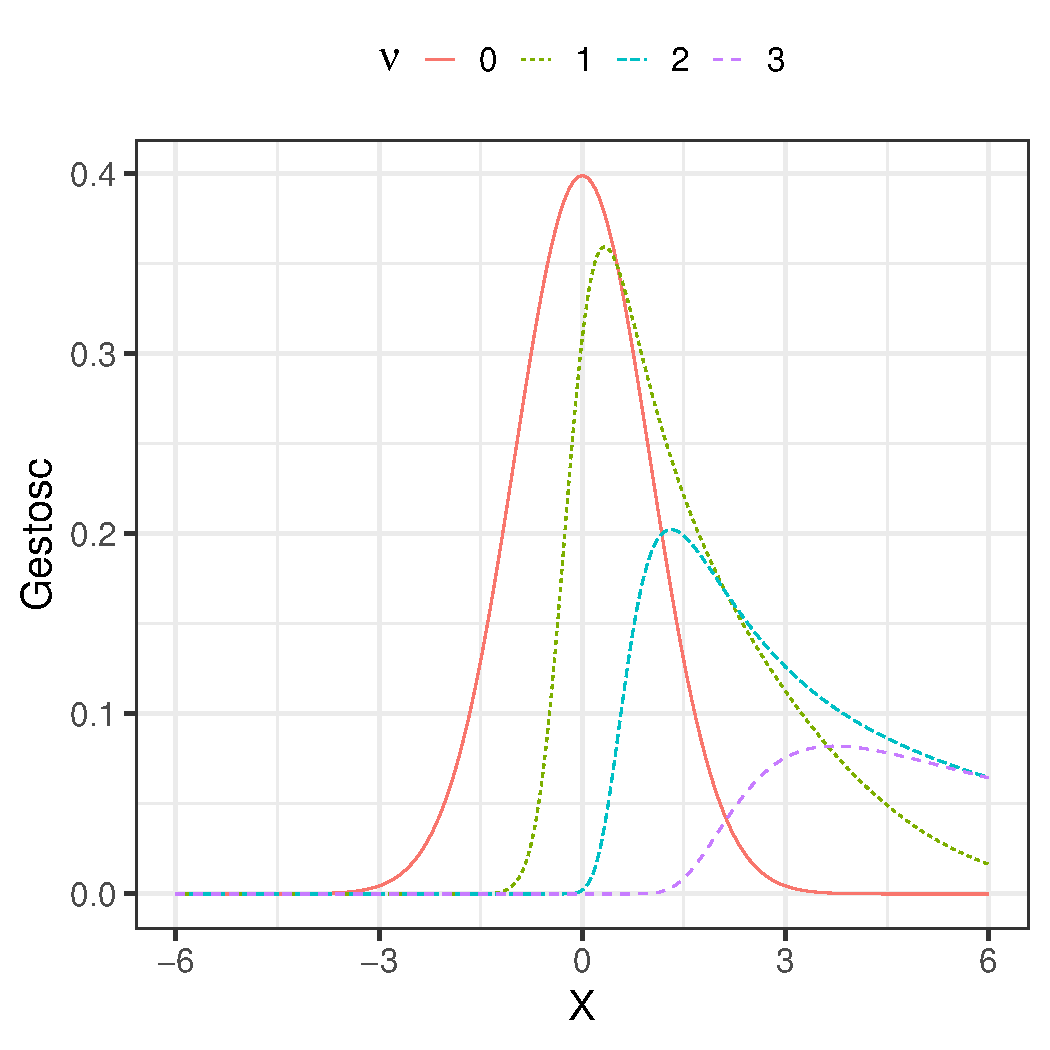
\includegraphics[scale=0.4]{skos.pdf}
				\caption{Transformata Sinh-arcsinh z modyfikacją $\nu$}
				\label{fig:skos}
			\end{minipage}
		\qquad \qquad
			\begin{minipage}{0.4\linewidth}
				\centering
				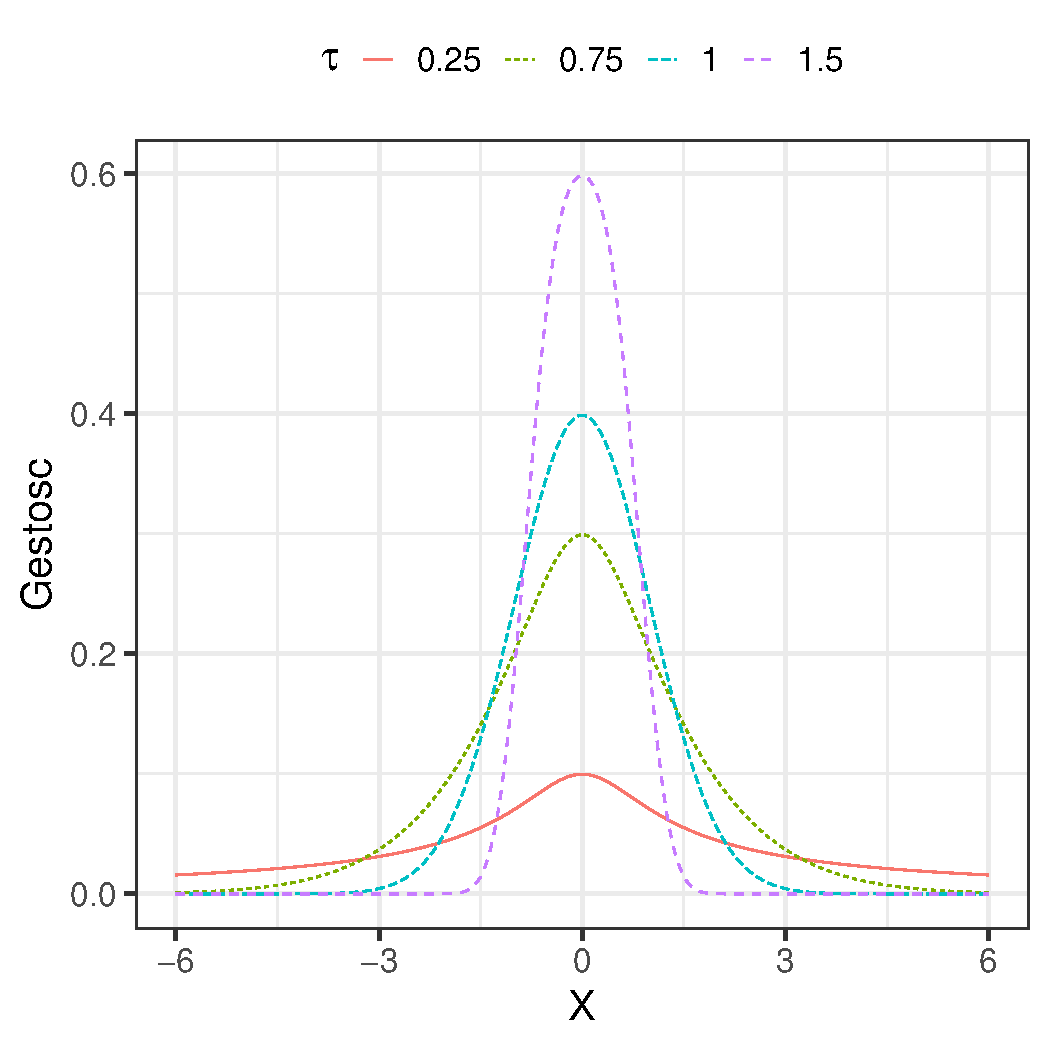
\includegraphics[scale=0.4]{kurt.pdf}
				\caption{Transformata Sinh-arcsinh z modyfikacja $\tau$}
				\label{fig:kurt}
			\end{minipage}
		\end{center}
	\end{figure}
Na rysunkach \ref{fig:skos}, \ref{fig:kurt} widzimy przykładowe rozkłady normalne po transformacji. Jak widać wartości $\nu > 0$ oznaczają rozkłady prawoskośne (analogicznie $\nu < 0$ będą lewoskośne), $\tau > 1$ oznacza rozkłady o chudszych ogonach niż normalny, natomiast $\tau < 1$ grubszych. Warto jednak podkreślić, że $\nu$ i $\tau$ nie są skośnością oraz kurtozą, jedynie parametrami kontrolującymi je nie wprost.
	W dalszej części raportu, sprawdzimy jak zmiany skośności oraz kurtozy wpływają na moc omawianych testów.
	
	\section{Wybrane testy statystyczne}
	Testy statystyczne mają zadanie oszacować prawdopodobieństwo spełnienia pewnej hipotezy statystycznej w populacji na podstawie próby losowej z tej populacji. W raporcie przyjrzymy się jak zmienia się moc wybranych testów normalności w obliczu transformaty sinh-arcsinh. Hipoteza zerowa $H_0$ którą przyjmujemy w każdym z nich brzmi: \textit{Próba pochodzi z rozkładu normalnego} przeciwko  hipotezie alternatywnej $H_1$: \textit{Próba nie pochodzi z rozkładu normalnego}.
	\subsection*{Test Shapiro-Wilka}
	Opiera się on na statystyce $W$, wyliczanej na podstawie danych z próbki, która będzie tym bliższa~1 im bardziej prawdopodobne jest to, że dane pochodzą z rozkładu normalnego.
	$$W = \frac{(\sum_{i=1}^{n}a_i x_{(i)})^2}{\sum_{i=1}^{n} (x_i - \bar{x})^2},$$
	gdzie $x_{{(i)}}$ z nawiasami w indeksie dolnym to i-ta najmniejsza liczba w próbie (nie mylić z $x_{i}$) a $\bar{x}$ oznacza średnią próbkową. Współczynniki $a_i$ dane są jako:
	$$(a_1, \dots, a_n) = \frac{m^T V^{-1}}{C},$$
	 gdzie $C$ jest wektorem norm:
	 $$C = \|V^{-1} m\| = (m^T V^{-1} V^{-1} m)^{\frac{1}{2}},$$
	 a wektor $m$:
	 $$m = (m_1,\dots,m_n)^T$$
	składa się z wartości oczekiwanych statystyki porządkowej (ang. \textit{order statistics}) niezależnych zmiennych losowych próbkowanych ze standardowego rozkładu normalnego, natomiast $V$ jest macierzą kowariancji tejże statystyki.
	
	\subsection*{Test Kołmogorowa-Lillieforsa}
	Statystyka tego testu, to maksymalna bezwzględna różnica między empiryczną a hipotetyczną funkcją rozkładu skumulowanego. Można obliczyć ją jako $D = D^+, D^-$, gdzie
	$$D^{+} = \max_{i=1,..., n}(i/n - p_{(i)}),\quad D^{-} = \max_{i=1,..., n}(p_{(i)} - (i-1)/n),$$
	gdzie: $$p_{(i)} = \Phi([x_{(i)} - \overline{x}]/s).$$ Tutaj $\Phi$ jest funkcją skumulowanego standardowego rozkładu normalnego, $\bar{x}$ i $s$ są średnią i odchyleniem standardowym wartości danych. 

	\subsection*{Test Jarque-Bera}
	 Jest to test dopasowania (ang. \textit{goodness of fit}), określający czy dane z próbki mają skośność i kurtozę odpowiadającą rozkładowi normalnemu. Statystyka $JB$ testu jest zawsze większa bądź równa zero. Jeżeli jest daleka od zera, sygnalizuje, że dane nie mają rozkładu normalnego.
	 $$JB = \frac{n}{6} \left( S^2 + \frac{1}{4} (K-3)^2 \right),$$
	 gdzie $n$ oznacza ilość obserwacji, natomiast $S$ oznacza skośność a $K$ kurtozę:
	 
	 $$S={\frac  {{\hat  {\mu }}_{3}}{{\hat  {\sigma }}^{3}}}={\frac  {{\frac  1n}\sum _{{i=1}}^{n}(x_{i}-{\bar  {x}})^{3}}{\left({\frac  1n}\sum _{{i=1}}^{n}(x_{i}-{\bar  {x}})^{2}\right)^{{3/2}}}},\qquad K={\frac {{\hat {\mu }}_{4}}{{\hat {\sigma }}^{4}}}={\frac {{\frac {1}{n}}\sum _{i=1}^{n}(x_{i}-{\bar {x}})^{4}}{\left({\frac {1}{n}}\sum _{i=1}^{n}(x_{i}-{\bar {x}})^{2}\right)^{2}}},$$
	 
	 Jeśli dane pochodzą z rozkładu normalnego, statystyka JB zbiega asymptotycznie do rozkładu chi kwadrat z dwoma stopniami swobody.
\section{Zadania}
	\subsection*{Zadanie 1}
	Dysponujemy próbą o rozmiarze 100 z rozkładu normalnego $\mathcal{N}(-1,3)$ przekształconego przez transformatę Sinh-arcsinh z $\nu = 0$. Na wykresie \ref{fig:z1} sprawdzamy jak zmiana parametru $\tau$ na przedziale $(0.5,2)$, wpływa na moc poszczególnych testów. Widzimy, że dla małych $\tau$ wszystkie testy radzą sobie dobrze. Niestety moc testu jest niska dla rozkładów leptokurtycznych i wzrasta powoli dla testów Kołmogorowa-Lillieforsa oraz Shapiro-Wilka. W przypadku testu Jarque-Bera moc testu pozostaje w przybliżeniu stała. Na zadanym przedziale nie ma testu jednostajnie najmocniejszego.
	\begin{figure}[H]
		\begin{center}
			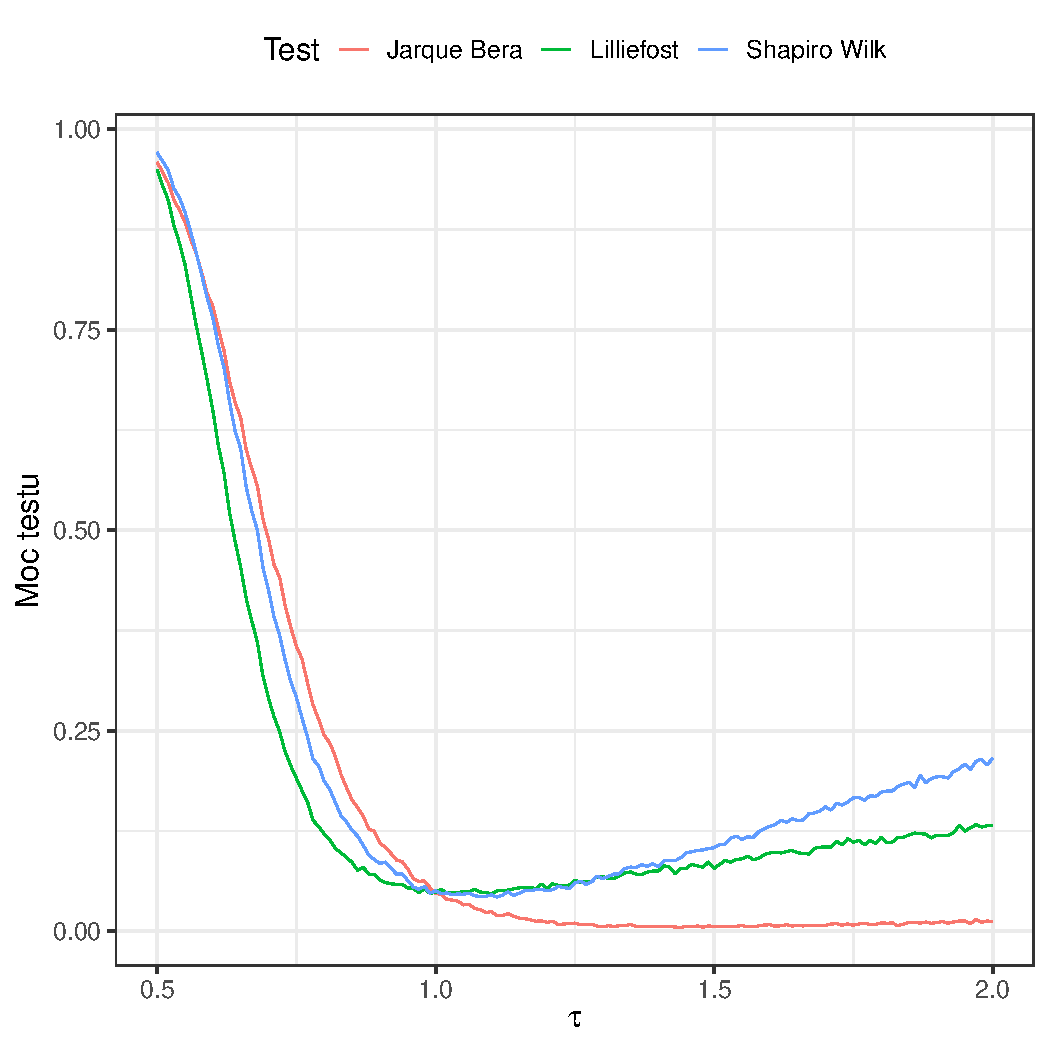
\includegraphics[scale=0.75]{zad1.pdf}
			\caption{Moc testu dla rozkładu Sinh-arcsinh wobec zmienności $\tau$}
			\label{fig:z1}
		\end{center}
	\end{figure}

	\subsection*{Zadanie 2}
	Dysponujemy próbą o rozmiarze 100 z rozkładu normalnego $\mathcal{N}(-1,3)$ przekształconego przez transformatę Sinh-arcsinh z $\tau = 1$. Na wykresie \ref{fig:z2} sprawdzamy jak zmiana parametru $\nu$ na przedziale $(-2,2)$, wpływa na moc poszczególnych testów. Zauważamy symetrię względem prostej $\nu = 0$. Wynika to z faktu, że dla przeciwnych $\nu$ skośność jest również przeciwna. Tym razem możemy wyróżnić jednostajnie najmocniejszy test - Shapiro-Wilka. Niemniej jednak na wyborze innych testów wiele nie stracimy.
	\begin{figure}[H]
		\begin{center}
			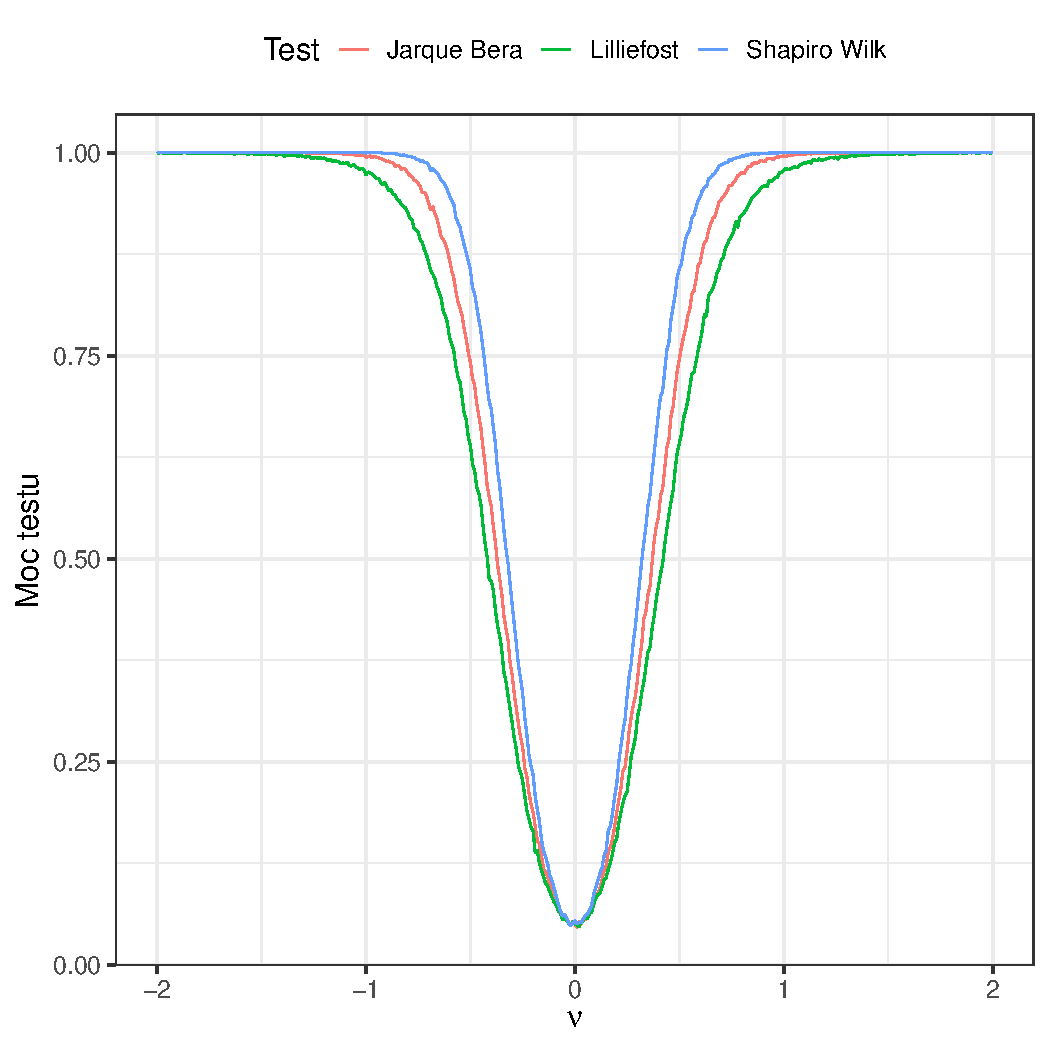
\includegraphics[scale=0.75]{zad2.pdf}
			\caption{Moc testu dla rozkładu Sinh-arcsinh wobec zmienności $\nu$}
			\label{fig:z2}
		\end{center}
	\end{figure}

	\subsection*{Zadanie 3}
	Mamy próbę $(X_1,\dots,X_{100})$ taką, że zmienne losowe $Y_i = \frac{X_i - 1}{3}$
	są z rozkładu t-Studenta $\mathcal{T}(\nu)$. Ponieważ $X_t$ jest liniową funkcją zmiennej z rozkładu t-Studenta oczekujemy, że wraz ze wzrostem liczby stopni swobody, jego rozkład będzie zbiegał do rozkłądu normalnego. Rzeczywiście, wykres \ref{fig:z3} potwierdza nasze przypuszczenia - moce testów zbiegają asymptotycznie do zera. Jednostajnie najmocniejszym testem jest test Jarque-Bera. Najgorzej spisuje się zaś test Kołmogorowa-Lillieforsa.
	\begin{figure}[H]
		\begin{center}
			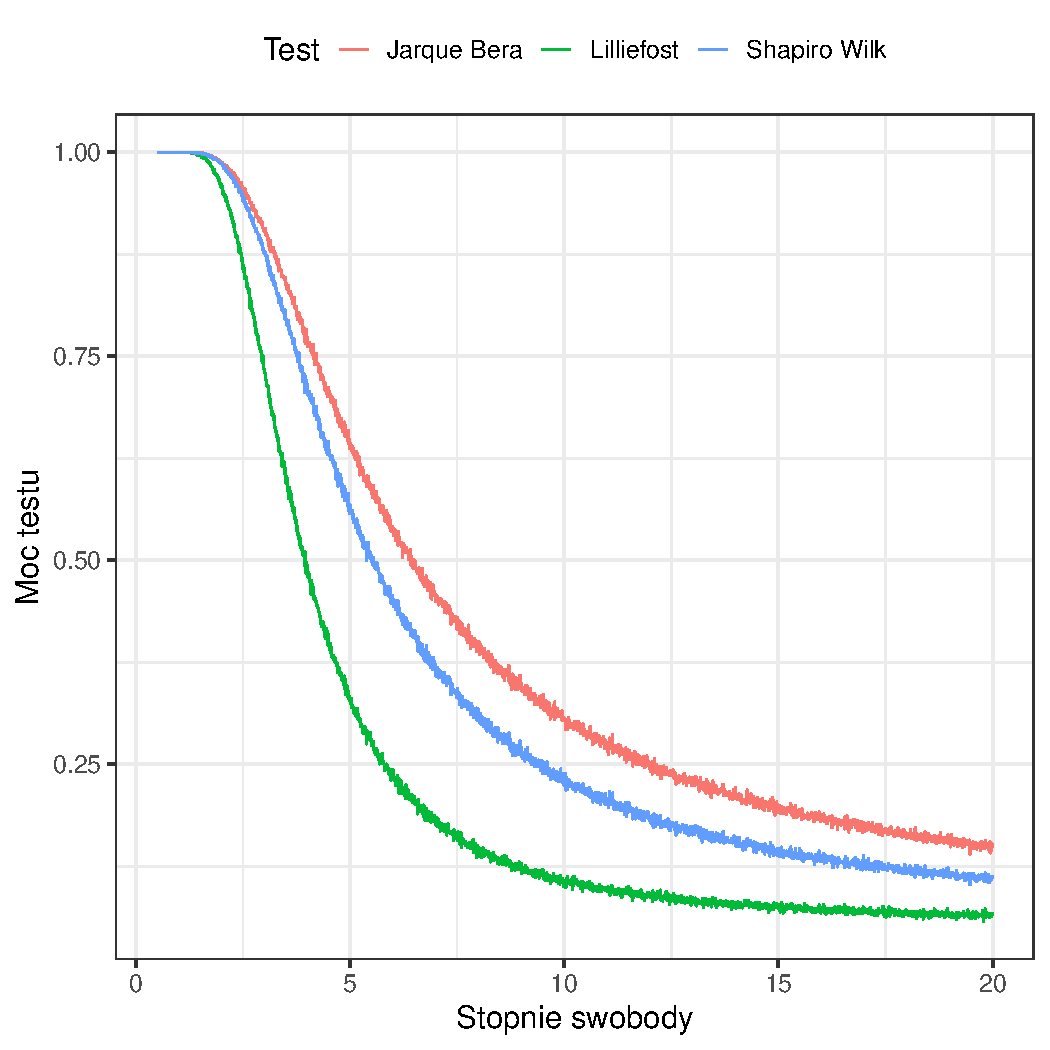
\includegraphics[scale=0.75]{zad3.pdf}
			\caption{Moc testu dla rozkładu t-Studenta wobec zmienności stopni swobody}
			\label{fig:z3}
		\end{center}
	\end{figure}

\section{Podsumowanie}
Rozwiązane zadania pokazały, że nie ma jednego uniwersalnego jednostajnie najmocniejszego testu. Wszystkie rozważane przez nas testy mają trudności w rozpoznaniu rozkładów podobnych do rozkładu normalnego. Przy testowaniu hipotez warto zatem wykonać kilka niezależnych testów oraz podchodzić do każdego przypadku indywidualnie.

\section{Źródłą}

\end{document}